\documentclass[../main.tex]{subfiles}

\begin{document}
    \subsection{面積の減少}
        プロセッサの面積を削減できると、
        一般的にチップあたりのコストを下げることができる。
        その影響で消費電力も低下することになる。
        よって今回はプロセッサの面積が削減できる改善方法を考えた.

        \subsubsection{マルチプレクサー}
        なぜマルチプレクサーの実装にこだわるか、論理合成をする時に気づいたことは、
        実際のプロセッサに「don't care 」の信号を論理的に考えると、
        この信号に対し、演算「比較、足し算など 」は無意味だと考えられる。
        例えば、分岐命令を考えると、
        WBステージにどのような値をレジスタファイルに書き込もうが、
        レジスタファイルへの書き込み制御信号を1「書き込まない」にすると、
        結局、その値は変化を持たさないので、
        この場面でのマルチプレクサーへの制御信号をどんな値にしても、
        結果的に、変わらないと思い、「」信号をプロセッサの状態への変化がない程度に
        0また1の信号を出力することにした。

        この原理を用いて、他のモジュールも書き換えることができた。
        さらに、この変化により、if-else文もVerilog-HDLにあるconditional operatorを用いて、簡単ができた。
        従って、面積を376773$\mu$$m^2$から268331$\mu$$m^2$まで、約29$\%$の面積が削減できた。

    \subsection{クリティカルパースの短縮} \label{ssec:aluImprove}
        データフォワーディングを1つのモジュールとして実装する前には、
        IDステージにある分岐先アドレスの加算機がクリティカルパースであった。
        さらに、分岐命令の時には、図\ref{fig:aluBefore}に示すように、
        ALUにある加算機は使われていないため、
        資源の無駄遣いかと考え、
        分岐条件の検証と同時に加算機を用いて、
        分岐先アドレスの計算も一緒に利用できないかと考えた。

        その解決は図\ref{fig:aluAfter}に示している。
        よって、IDステージにあるクリティカルパースは解決できた。
        ただし、データフォワーディングを1つのモジュールとして、実装してから、
        新たなクリティカルパースとして、問題になった。
        これの改善方法は\ref{ssec:forwardingImprove}に詳しく述べる。

        \begin{figure}[h]
            \centering
            \begin{subfigure}{\columnwidth}
                \centering
                
\includegraphics[width = 1.3\columnwidth]{../images/old_alu.png}
                \caption{改善前のALU}
                \label{fig:aluBefore}
            \end{subfigure}
            \begin{subfigure}{\columnwidth}
                \centering
                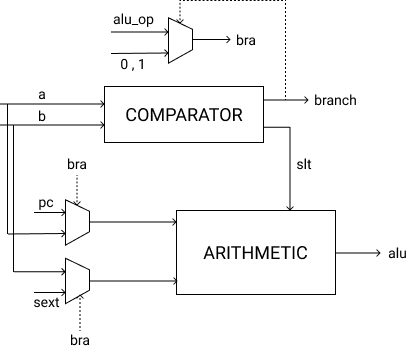
\includegraphics[width = 1.3\columnwidth]{../images/new_alu.jpg}
                \caption{改善後のALU}
                \label{fig:aluAfter}
            \end{subfigure}
            \caption{ALUでの改善}
            \label{fig:aluImprove}
        \end{figure}

\end{document}
